Anche in caso di guasti:
\begin{itemize}
    \item gli effetti delle transazioni \textbf{committed} devono essere permanenti (Durability)
    \item gli effetti delle transazioni \textbf{aborted} non devono lasciare tracce (Atomicity)
\end{itemize}
In caso di guasti quindi il gestore del ripristino deve deve identificare i malfunzionamenti e ripristinare la base di dati allo stato (consistente) precedente il malfunzionamento.\\
II tipi di malfunzionamenti sono essenzialmente 3:
\begin{itemize}
    \item \textbf{Transaction Failure}: Transazione abortisce.
    \item \textbf{System failure}: Guasto Hardware che non danneggia la memoria permanente.
    \item \textbf{Media (o device) failure}: Contenuto della base di dati danneggiato.
\end{itemize}
Classificazione delle memorie:
\begin{itemize}
    \item \textbf{Memoria volatile}: le informazioni contenute vengono perse in caso di cadute di sistema (RAM)
    \item \textbf{Memoria non volatile}: le informazioni contenute sopravvivono a cadute di sistema, possono però essere perse a causa di altri malfunzionamenti (HDD)
    \item \textbf{Memoria stabile}: le informazioni contenute non possono essere perse (astrazione teorica)
\end{itemize}
\begin{figure}[H]
    \centering
    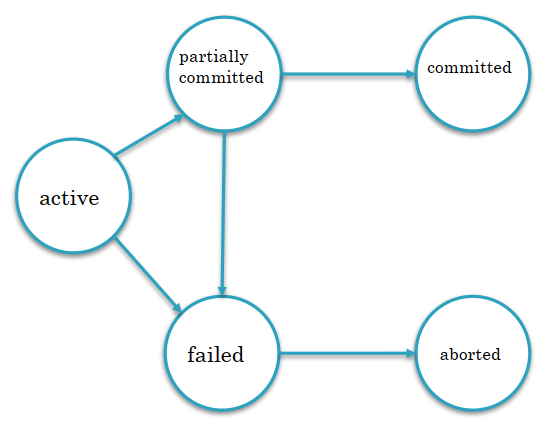
\includegraphics[width=0.6\textwidth, keepaspectratio]{ModelloDiEsecuzione.png}
    \label{fig:ModelloDiEsecuzione}
\end{figure}
I nodi "committed" e "aborted" sono raggiunti solo dopo che l'operazione e lo stato precedente \`e stato "ufficializzato" in memoria persistente.

\break
\noindent Dopo un rollback di una transazione, il sistema può:
\begin{itemize}
    \item \textbf{rieseguire la transazione}: ha senso solo se la transazione è stata abortita a seguito di errori software o hardware non dipendenti dalla logica interna della transazione
    
    \item \textbf{eliminare la transazione}: se si verificano transaction failures che possono essere corretti solo riscrivendo il programma applicativo
\end{itemize}

\subsection{Recovery con log (Ripresa a caldo)}
Utilizza un file di log in memoria stabile dove vengono registrate sequenzialmente le operazioni di ogni transazione con riferimento all'operazione precedente. Questo permette di fare operazioni di \code{REDO/UNDO} in caso di failure.\\
Struttura di un record del log:
\begin{center}
    (\underline{LSN}, T, PID, before(P), after(P), prevLSN)
\end{center}
\begin{itemize}
    \item \textbf{LSN}: Log Sequence Number
    \item \textbf{T}: Identificatore Transazione
    \item \textbf{PID}: Page ID modificata
    \item \textbf{before}: "before image", continuto prima della modifica
    \item \textbf{after}: "after image"
    \item \textbf{prevLSN}: LSN del record id log precedente di T
\end{itemize}
\begin{figure}[H]
    \centering
    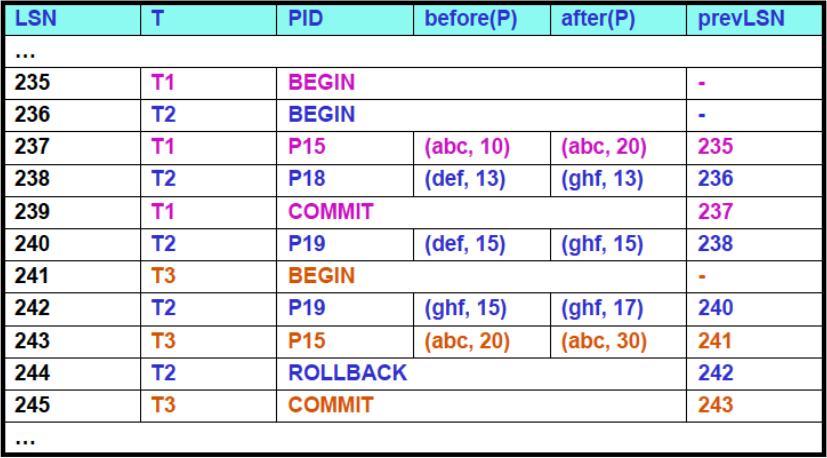
\includegraphics[width=0.8\textwidth, keepaspectratio]{log1.png}
    \label{fig:log1}
\end{figure}
Per assicurare che il log possa essere usato in maniera corretta \`e importante applicare il protocollo \textbf{WAL} (Write Ahead Logging):\\
\textbf{Prima di scrivere su disco una pagina P modificata, il corrispondente Log record deve essere già stato scritto nel Log}\\
Una transazione si considera committed solo quando tutti i suoi record di log sono stati salvati su memoria stabile!

\break
\noindent Quindi l'ordine di esecuzione \`e il seguente:
\begin{enumerate}
    \item comando di Update
    \item creazione record di log
    \item scrittura del record di log sul disco
    \item scrittura della madifica su disco
\end{enumerate}

\subsubsection{Gestione del buffer}
Ci sono 2 politiche per decidere quando scrivere la pagina modificata su disco:
\begin{itemize}
    \item \textbf{No Steal}: Si mantiene la pagina P nel buffer fino al \code{COMMIT}
    \item \textbf{Steal}: Si scrive P quanto si può o conviene (per liberare il buffer ad esempio) anche prima del \code{COMMIT}
\end{itemize}
Nel caso di \textbf{No Steal} non ci sarà mai bisogno di fare un UNDO ma si usa molta più RAM.\vspace{2mm} \\
Ci sono inoltre 2 politiche per quando registrare il \code{COMMIT}:
\begin{itemize}
    \item \textbf{Force}: Si forza la scrittura prima di scrivere il record di \code{COMMIT} nel Log
    \item \textbf{No Force}: Si scrive il record di \code{COMMIT} nel log subito.
\end{itemize}
Con la politica \textbf{No Force} la pagina viene scritta sul disco solo deve essere rimpiazzata nel buffer riducendo le operazioni di I/O.\vspace{4mm} \\
\textbf{Riassunto in caso di Failure:}
\begin{itemize}
    \item \textbf{STEAL}: Log a modifiche immediate, serve procedura di UNDO
    
    \item \textbf{NO STEAL}: Log a modifiche differite, inutile mantenere anche la versione vecchia dei dati perché gli aggiornamenti non dovranno mai essere disfatti
    
    \item \textbf{NO FORCE}: Serve procedura di REDO
    
    \item \textbf{FORCE}: Non serve procedura di REDO perché al commit i dati saranno già tutti copiati su disco (e se una transazione non è arrivata al commit deve solo essere disfatta)
\end{itemize}
La combinazione più comune \`e: steal-no force (undo se non è arrivata al commit, redo se è arrivata al commit)

\subsubsection{Checkpoint}
Un checkpoint \`e una scrittura forzata su disco delle pagine modificate e viene registrata sul log come \code{CKP}. Se T ha eseguito il commit prima del checkpoint siamo certi che sia stata completata.\\
Periodicamente quindi il DBMS esegue:
\begin{itemize}
    \item forza tutte le pagine di log residenti in memoria principale su memoria stabile
    \item forza tutte le pagine dati di buffer su disco
    \item forza il record $<$CKP$>$ (o $<$checkpoint$>$) sul log in memoria stabile
\end{itemize}
Questo riduce i tempi relativi alla procedura di restart.

\subsection{Media failure (Ripresa a freddo)}
Per far fronte a malfunzionamenti della memoria non volatile serve un altra procedura rispetto al log: il \textbf{dump}.\\
\textbf{Dump}: copia completa della base di dati, normalmente creata quando il sistema non è operativo (nessuna transazione in esecuzione)\\
La copia è memorizzata in memoria stabile, ed è chiamata \textbf{backup}.\\
Un record <dump> nel log segnala la presenza di un backup effettuato in un certo momento ed identifica il file o il device su cui è stato effettuato il dump.\vspace{2mm}\\
La procedura per una ripresa a freddo \`e:
\begin{enumerate}
    \item Al restart, si accede al dump e si ripristina il contenuto della base di dati su memoria non volatile
    \item Si effettua una ripresa a caldo: si accede il file di log e si esegue il ripristino come discusso in precedenza
\end{enumerate}